\section{Grafiek 1}

\begin{figure}[!htb]
    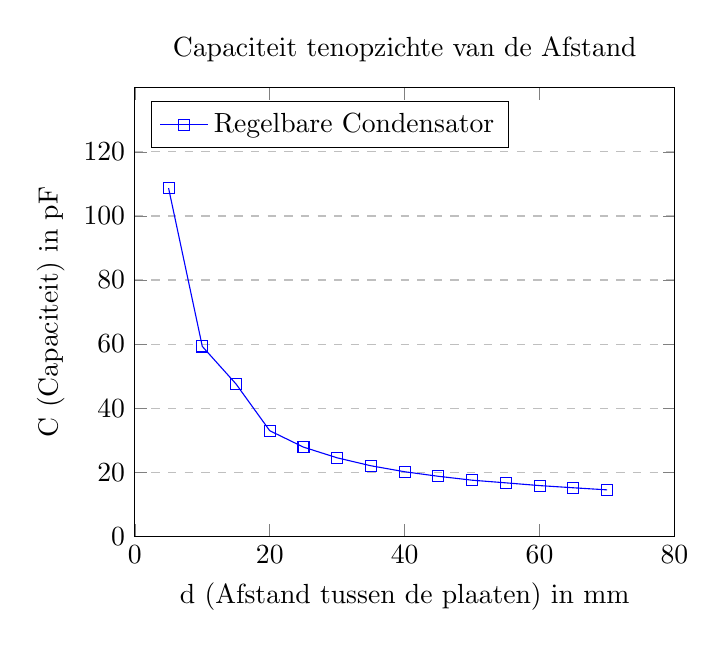
\begin{tikzpicture}
        \begin{axis}[
            title={Capaciteit tenopzichte van de Afstand},
            xlabel={d (Afstand tussen de plaaten) in mm},
            ylabel={C (Capaciteit) in pF},
            xmin=0, xmax=80,
            ymin=0, ymax=140,
            xtick={0,20,40,60,80},
            ytick={0,20,40,60,80,100,120},
            legend pos=north west,
            ymajorgrids=true,
            grid style=dashed,
        ]
        
        \addplot[
            color=blue,
            mark=square,
            ]
            coordinates {
            (5,108.68)(10,59.261)(15,47.529)(20,32.933)(25,27.814)(30,24.469)(35,21.987)(40,20.125)(45,18.704)(50,17.487)(55,16.658)(60,15.802)(65,15.121)(70,14.468)
            };
            \legend{Regelbare Condensator}
            
        \end{axis}
    \end{tikzpicture}
\end{figure}